\documentclass[11pt, titlepage,a4paper]{article}
\usepackage[utf8]{inputenc}
\usepackage{natbib}
\usepackage{hyperref}
\usepackage{dsfont}
\usepackage{subfigure}
\usepackage{multicol}
\usepackage[T1]{fontenc}
\usepackage[left=2cm,right=2cm,top=2cm,bottom=2cm]{geometry}
\usepackage[spanish, activeacute]{babel}
\usepackage{amsmath}
\usepackage{amssymb,amsfonts,textcomp}
\usepackage{color}
\usepackage{array}
\usepackage{hhline}
\usepackage{varwidth}
\usepackage{graphicx}
\usepackage{parcolumns}
\usepackage{cite}
\usepackage{hyperref}
\usepackage[]{algorithm2e}


\hypersetup{ colorlinks=true, linkcolor=black, citecolor=black, filecolor=black,
urlcolor=blue, pdftitle=Laboratorio 6: Clustering Jerarquico , pdfauthor= Alberto Fernández Arkaitz Marcos Endika Serrano}

\bibliographystyle{plain}


\renewcommand{\thefootnote}{\fnsymbol{footnote}}
\title{\textbf{\huge{Mineria de Datos} \\Laboratorio 6: Clustering
Jerarquico \newline
\begin{center}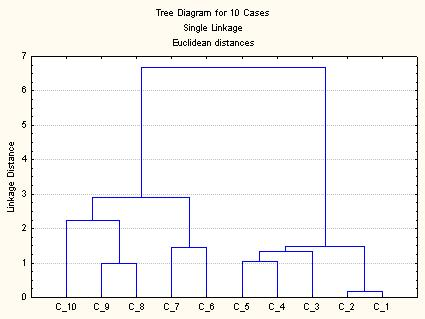
\includegraphics[scale =
1.4]{./images/Portada.jpg}\newline\footnote{Imagen extraida de
\url{http://jmj-qa.blogspot.com.es/2011/09/analisis-cluster.html}}\end{center}}
}


\author{Alberto Fernández \and Arkaitz Marcos \and Endika Serrano}
\date{}

\begin{document}
\maketitle

\tableofcontents

\newpage
\renewcommand{\thefootnote}{\arabic{footnote}}

\section{Introducción}

El objetivo de esta práctica es la programación de un algoritmo de clustering
jerárquico evitando la utilización de librerías de terceros y tratando de
mejorar el rendimiento frente a programas de minería de datos de uso general
como puede ser \textbf{Weka}.


\subsection{Definición}
 
\paragraph{Clasificación no-supervisada:\\}
Los métodos de clasificación en los que los datos de entrenamiento son vectores
x sin una clase definida.
\cite{Bishop}, Página 3, 2º Párrafo

La clasificación no supervisada tiene como objetivo la agrupación de datos en
grupos, estas agrupaciones tienen valor por sí mismas y su clasificación no
tiene interés.para ello emplea la similitud/disimilitud entre los atributos de
las distintas instancias para poder realizar la “clasificación” sin contar con
la clase definida que le indique la clasificación correcta o el grado de error
en las distintas predicciones.\cite{Elements} , Página 486,
3ºlinea \[\cite{Handbook}, Sección 14.1, 1º Párrafo\]

\subsection{Objetivo}
El objetivo de esta práctica es el diseño e implementación de un algoritmo de
clasificación no supervisada mediante la técnica del Clustering Jerárquico,
tanto en su variante  como Aglomerativa como Divisiva evitando la utilización de
librerías de terceros.

\bigskip

Hemos utilizado principalmente los siguientes archivos:

\begin{description}
\item[color.arff]Este fichero cuenta con 62 instancias y 2001 atributos
numéricos junto con la clase nominal.
\item[food.arff]Este fichero cuenta con 24 instancias y 6 atributos, de los
cuales 5 son numéricos y 1 de tipo string.
\end{description}

\section{Algoritmo}
\subsection{Aglomerativo}
\begin{center}
\fbox{%
\begin{varwidth}{\dimexpr\linewidth-2\fboxsep-2\fboxrule\relax}
\begin{enumerate}
\item iteration $\leftarrow$ 1 
\item while \{iteration < nº Instancias\}

\subitem merge the best 2 clusters (the nearest) and add it in the cluster
list after removing the merged clusters

\subitem create a new Iteration including the new cluster list

\subitem add the new Iteration to the last position of the list of
iterations

\item do iteration $\leftarrow$ iteration +1 

\end{enumerate}
	\end{varwidth}% 
		
	}
\end{center}
%Clustering jerarquico en pseudocodigo

\subsection{Divisivo}
\begin{center}

\fbox{%
\begin{varwidth}{\dimexpr\linewidth-2\fboxsep-2\fboxrule\relax}
\begin{enumerate}
\item iteration $\leftarrow$ 1 
\item while \{iteration < nº Instancias\}

\subitem divide the best clusters (the furthest instances in the cluster) and
add the new cluster to the cluster list

\subitem create a new Iteration including the new cluster list

\subitem add the new Iteration to the last position of the list of
iterations

\item do iteration $\leftarrow$ iteration +1 

\end{enumerate}
	\end{varwidth}% 
		
	}
\end{center}

\section{Diseño}
\begin{figure}[hbtp]
\centering
\includegraphics[scale = 0.18]{images/DiagramaP}
\end{figure}

Si no pongo esto ahora el titulo se queda por debajo
\section{Resultados experimentales}

\subsection{Banco de pruebas}

\subsection{Resultados obtenidos}

\subsection{Resultados respecto a otro software}

\subsection{Análisis de resultados}

\subsection{Rendimiento del software}

\section{Conclusiones}

\section{Bibliografía}

\bibliography{bibliografia}

%\section{Valoración subjetiva}
\end{document}